\documentclass{standalone}
\usepackage{tikz}
\begin{document}
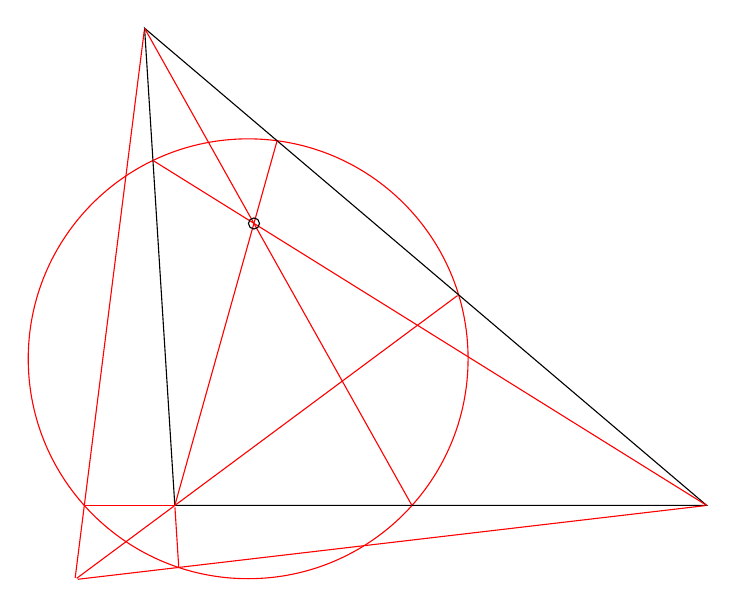
\begin{tikzpicture}[x=1pt,y=1pt]
\draw[red] (49.17,-195.45) -- (81.43,-195.45);
\draw[red] (83.07,-217.87) -- (81.70,-196.20);
\draw[red] (108.15,-142.45) circle (79.47);
\draw (81.65,-195.45) -- (273.86,-195.45) -- (70.72,-23.01) -- cycle;
\draw[red] (45.64,-221.64) -- (70.61,-23.85);
\draw[red] (46.59,-222.13) -- (273.29,-195.52);
\draw[red] (46.20,-221.78) -- (183.80,-119.61);
\draw[red] (70.72,-23.01) -- (167.34,-195.47);
\draw[red] (273.86,-195.45) -- (73.75,-70.79);
\draw[red] (81.65,-195.45) -- (118.61,-63.66);
\draw (110.25,-93.56) circle (2.00);
\end{tikzpicture}
\end{document}
